\documentclass[10pt,english,a4paper]{article}
\newcommand{\dir}{.}
\newcommand{\commondir}{../common}
\input{\commondir/packages.tex}
\usepackage{color}
\usepackage[colorlinks=true,citecolor=blue,dvipdfm]{hyperref}
\input{\commondir/definitions.tex}



\pagestyle{myheadings}

\markright{Glimmer-CISM Branches}

\begin{document}
\title{Glimmer-CISM Branches}
\author{Magnus Hagdorn\thanks{Magnus.Hagdorn@ed.ac.uk}}

\maketitle

2010 will be an exciting year for Glimmer-CISM development. We plan to make a release of the model with the higher order physics included. There are also plans for a major refactoring effort to make the ice sheet model more modular.

\begin{figure}[htbp]
\centering
\includegraphics[width=\textwidth]{\dir/figs/gc-branches.eps}
\caption{Glimmer-CISM branches and merge points for 2010}
\end{figure}

The diagram above illustrates the relationship among various existing branches and branches to be created. We have the following plans:
\begin{enumerate}
\item create a preview snapshot of the Glimmer-CISM-lanl branch in February
\item Magnus Hagdorn will merge the Glimmer-CISM-lanl branch into Glimmer-CISM2-trunk after it has been finalised. The Glimmer-CISM-lanl branch will cease to be active.
\item make a release of Glimmer-CISM2-trunk which includes the higher order physics. This will become Glimmer-CISM-1.8-stable series. Aim for a release in time for EGU in May.
\item merge Glimmer-CISM2-trunk into Glimmer-CISM-2-refactoring so that it contains the higher order physics. Continue refactoring. This should happen after version 1.8 has been released
\item Once we are happy with the refactoring merge it back into Glimmer-CISM-2-trunk. Glimmer-CISM-2-refactoring will become inactive. This might happen in autumn?
\item Once we are ready, create a new stable series containing higher order physics and refactored code.
\item Bill will update the version of Glimmer used by CCSM to the latest version in the 1.0 series.
\end{enumerate}

\end{document}
